\documentclass[12pt]{article}
\usepackage{amsmath}
\usepackage{graphicx}
\usepackage{hyperref}
\usepackage{listings}
\usepackage{color}
\usepackage{pythonhighlight}

\title{Operating System Course Report - First Half of the Semester}
\author{A class}
\date{\today}

\begin{document}

\maketitle
\newpage

\tableofcontents
\newpage

\section{Introduction}
This report summarizes the topics covered during the first half of the Operating System course. It includes theoretical concepts, practical implementations, and assignments. The course focuses on the fundamentals of operating systems, including system architecture, process management, CPU scheduling, and deadlock handling.

\section{Course Overview}
\subsection{Objectives}
The main objectives of this course are:
\begin{itemize}
    \item To understand the basic components and architecture of a computer system.
    \item To learn process management, scheduling, and inter-process communication.
    \item To explore file systems, input/output management, and virtualization.
    \item To study the prevention and handling of deadlocks in operating systems.
\end{itemize}

\subsection{Course Structure}
The course is divided into two halves. This report focuses on the first half, which covers:
\begin{itemize}
    \item Basic Concepts and Components of Computer Systems
    \item System Performance and Metrics
    \item System Architecture of Computer Systems
    \item Process Description and Control
    \item Scheduling Algorithms
    \item Process Creation and Termination
    \item Introduction to Threads
    \item File Systems
    \item Input and Output Management
    \item Deadlock Introduction and Prevention
    \item User Interface Management
    \item Virtualization in Operating Systems
\end{itemize}

\section{Topics Covered}

\subsection{Basic Concepts and Components of Computer Systems}
This section explains the fundamental components that make up a computer system, including the CPU, memory, storage, and input/output devices.

\subsection{System Performance and Metrics}
\subsection{Performa Sistem dan Metrik Sistem Komputer}
\subsubsection{Performa Sistem}
    Performa sistem komputer adalah kemampuan suatu sistem untuk menjalankan tugas-tugas komputasi sesuai dengan spesifikasi dan parameter yang telah ditetapkan. Performa ini mencakup kecepatan, efisiensi, dan ketepatan dalam menyelesaikan berbagai proses dan operasi yang diminta oleh pengguna atau aplikasi.
\begin{enumerate}
    \item {Faktor Pengaruh performa}
    \par \begin{enumerate}
        \item {CPU (\textit{(Central Processing Unit)}}
        \par CPU atau prosesor adalah otak dari komputer yang bertanggung jawab untuk menjalankan instruksi dan proses komputasi. Kecepatan \textit{CPU} diukur dalam \textit{gigahertz (GHz)}; semakin tinggi frekuensi, semakin cepat proses eksekusi instruksi. Jumlah \textit{core} pada CPU juga penting; semakin banyak \textit{core}, semakin baik komputer dalam menangani \textit{multitasking} dan aplikasi yang membutuhkan banyak sumber daya\cite{3.2.1 Vaia}.
        \item {GPU \textit{(Graphics Processing Unit)}}
        \par GPU bertanggung jawab untuk menangani pemrosesan grafis dan rendering visual. Dalam aplikasi yang memerlukan performa grafis tinggi seperti game dan desain 3D, GPU yang kuat menjadi sangat penting. GPU modern juga digunakan untuk komputasi paralel di bidang kecerdasan buatan dan pembelajaran mesin, GPU dapat menyelesaikan tugas sederhana dan berulang jauh lebih cepat karena dapat memecah tugas menjadi komponen yang lebih kecil dan menyelesaikannya secara paralel\cite{3.2.1 AWS. GPU vs CPU}.
        
        \item {RAM \textit{(Random Access Memory)}}
        \par RAM adalah memori sementara yang digunakan oleh sistem untuk menyimpan data yang aktif digunakan atau diakses oleh CPU dengan cepat. Jumlah dan kecepatan RAM biasanya meningkatkan performa sistem dengan memungkinkan lebih banyak data digunakan tanpa harus menggunakan penyimpanan yang lebih lambat\cite{3.2.1 Algor Cards}.

    \end{enumerate}
    
    \item {Keterkaitan Hardware}
    \par \begin{enumerate}
        \item {Keterkaitan antara RAM dan CPU}
        \par CPU bergantung pada RAM untuk menyimpan data sementara yang sedang diproses. Ketika CPU menjalankan tugas, ia membutuhkan data yang dapat diakses dengan cepat. RAM menyediakan ruang penyimpanan sementara yang memungkinkan CPU untuk mengakses data dengan kecepatan tinggi, yang membantu mencegah penundaan dalam pemrosesan. Semakin besar kapasitas dan kecepatan RAM, semakin cepat CPU dapat memproses data, terutama dalam situasi \textit{multitasking} ketika banyak aplikasi berjalan secara bersamaan.
    
        \item {Keterkaitan antara CPU dan GPU}
        \par CPU dan GPU bekerja bersama-sama untuk membagi tugas yang memerlukan pemrosesan berat. CPU menangani tugas-tugas umum seperti logika, kontrol aplikasi, dan aliran data, sementara GPU menangani tugas-tugas yang membutuhkan komputasi paralel, seperti rendering grafis atau komputasi numerik. Kinerja keseluruhan sistem meningkat ketika CPU dan GPU dapat bekerja secara seimbang. Jika salah satu komponen terlalu lambat dibandingkan dengan yang lain, bisa terjadi \textit{bottleneck}, ketika salah satu perangkat keras menahan kinerja perangkat lainnya.
    
        \item {Keterkaitan antara Penyimpanan dan RAM}
        \par RAM dan penyimpanan juga bekerja sama untuk memastikan kelancaran operasi sistem. Ketika aplikasi atau data yang dibutuhkan oleh CPU tidak dapat seluruhnya ditampung di RAM, sistem akan menggunakan penyimpanan sebagai memori virtual. Jika penyimpanan yang digunakan adalah SSD (\textit{Solid State Drive}), maka akses data dari penyimpanan ke RAM menjadi jauh lebih cepat dibandingkan dengan HDD (\textit{Hard Disk Drive}) tradisional, sehingga mempercepat pemuatan aplikasi dan respons sistem secara keseluruhan.
    
    \end{enumerate} 

\end{enumerate}

\subsection{System Architecture of Computer Systems}
Describes the architecture of modern computer systems, focusing on the interaction between hardware and the operating system.

\subsection{Process Description and Control}
Processes are a central concept in operating systems. This section covers:
\begin{itemize}
    \item Process states and state transitions
    \item Process control block (PCB)
    \item Context switching
\end{itemize}

\subsection{Scheduling Algorithms}
This section covers:
\begin{itemize}
    \item First-Come, First-Served (FCFS)
    \item Shortest Job Next (SJN)
    \item Round Robin (RR)
\end{itemize}
It explains how these algorithms are used to allocate CPU time to processes.

\subsection{Process Creation and Termination}
Details how processes are created and terminated by the operating system, including:
\begin{itemize}
    \item Process spawning
    \item Process termination conditions
\end{itemize}

\subsection{Introduction to Threads}
This section introduces the concept of threads and their relation to processes, covering:
\begin{itemize}
    \item Single-threaded vs. multi-threaded processes
    \item Benefits of multithreading
\end{itemize}

\begin{figure}[h]
    \centering
    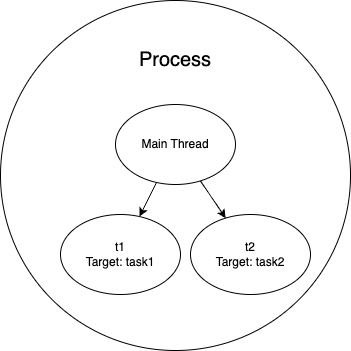
\includegraphics[width=0.5\textwidth]{/Users/khawaritzmi/Unhas/os_report_mid2024/a_class/asset/example.png}  % Sesuaikan nama file dan ukurannya
    \caption{Ini adalah gambar contoh dari multithreading.}
    \label{fig:contoh_gambar}
\end{figure}

Seperti yang terlihat pada Gambar \ref{fig:contoh_gambar}, inilah cara menambahkan gambar dengan keterangan.

\subsection{File Systems}
File systems provide a way for the operating system to store, retrieve, and manage data. This section explains:
\begin{itemize}
    \item File system structure
    \item File access methods
    \item Directory management
\end{itemize}

\subsection{Input and Output Management}
Input and output management is key for handling the interaction between the system and external devices. This section includes:
\begin{itemize}
    \item Device drivers
    \item I/O scheduling
\end{itemize}

\subsection{Deadlock Introduction and Prevention}
Explores the concept of deadlocks and methods for preventing them:
\begin{itemize}
    \item Deadlock conditions
    \item Deadlock prevention techniques
\end{itemize}

\subsection{User Interface Management}
This section discusses the role of the operating system in managing the user interface. Topics covered include:
\begin{itemize}
    \item Graphical User Interface (GUI)
    \item Command-Line Interface (CLI)
    \item Interaction between the user and the operating system
\end{itemize}

\subsection{Virtualization in Operating Systems}
Virtualization allows multiple operating systems to run concurrently on a single physical machine. This section explores:
\begin{itemize}
    \item Concept of virtualization
    \item Hypervisors and their types
    \item Benefits of virtualization in modern computing
\end{itemize}

\section{Assignments and Practical Work}
\subsection{Assignment 1: Process Scheduling}
\subsubsection{Group 2}
\textbf{Soal:}
    \par Buatlah sebuah program Python sederhana yang dapat mensimulasikan algoritma penjadwalan proses dengan menggunakan Round Robin Scheduling. Program ini harus mendukung beberapa fitur berikut:
    \begin{itemize} 
    \item Menerima daftar proses dengan burst time masing-masing.
    \item Mengatur proses dengan kuantum waktu tetap.
    \item Menampilkan urutan eksekusi proses serta waktu selesai masing-masing.
    \item Hitung waktu rata-rata turnaround time dan waiting time.
    \end{itemize}

\textbf{Jawaban:}
    Untuk menyelesaikan soal ini, berikut adalah implementasi dari algoritma Round Robin Scheduling sederhana dalam Python:

\begin{python} def round_robin(processes, burst_time, quantum): n = len(processes) remaining_time = burst_time[:] # Salin burst time awal waiting_time = [0] * n turnaround_time = [0] * n t = 0 # Waktu berjalan

python
Copy code
    while True:
        done = True
        for i in range(n):
            if remaining_time[i] > 0:
                done = False  # Ada proses yang belum selesai
                if remaining_time[i] > quantum:
                    t += quantum
                    remaining_time[i] -= quantum
                else:
                    t += remaining_time[i]
                    waiting_time[i] = t - burst_time[i]
                    remaining_time[i] = 0
        if done:
            break

    # Hitung turnaround time
    for i in range(n):
        turnaround_time[i] = burst_time[i] + waiting_time[i]

    print("Proses\tBurst Time\tWaiting Time\tTurnaround Time")
    for i in range(n):
        print(f"{processes[i]}\t{burst_time[i]}\t\t{waiting_time[i]}\t\t{turnaround_time[i]}")

    print(f"\nRata-rata Waiting Time: {sum(waiting_time) / n:.2f}")
    print(f"Rata-rata Turnaround Time: {sum(turnaround_time) / n:.2f}")

if __name__ == "__main__":
    processes = ['P1', 'P2', 'P3']
    burst_time = [24, 3, 3]
    quantum = 4
    round_robin(processes, burst_time, quantum)
\end{python}

\subsection{Assignment 2: Deadlock Handling}
In this assignment, students were asked to simulate different deadlock scenarios and explore various prevention methods.

\subsection{Assignment 3: Multithreading and Amdahl's Law}
This assignment involved designing a multithreading scenario to solve a computationally intensive problem. Students then applied **Amdahl's Law** to calculate the theoretical speedup of the program as the number of threads increased.

\subsection{Assignment 4: Simple Command-Line Interface (CLI) for User Interface Management}
Students were tasked with creating a simple **CLI** for user interface management. The CLI should support basic commands such as file manipulation (creating, listing, and deleting files), process management, and system status reporting.

\subsection{Assignment 5: File System Access}
\subsubsection{Group 2}
    \textbf{Soal:}
    \par Buatlah sebuah program Python sederhana untuk melakukan akses sistem file. Program ini harus mendukung beberapa perintah berikut:
    \begin{itemize}
    \item Membaca isi file teks.
    \item Menambahkan teks ke dalam file yang sudah ada.
    \item Menampilkan status akses file, seperti siapa pemiliknya, waktu modifikasi terakhir, dan izin akses file.
    \end{itemize}
    
    \textbf{Jawaban:}
    Berikut adalah implementasi dari program Python yang dapat mengakses sistem file dan mendukung fitur-fitur yang diminta:
    
    \begin{python} import os import stat from datetime import datetime
    
    python
    Copy code
    def baca_file(nama_file):
        try:
            with open(nama_file, 'r') as f:
                print(f"\nIsi file '{nama_file}':")
                print(f.read())
        except FileNotFoundError:
            print(f"File '{nama_file}' tidak ditemukan.")
        except Exception as e:
            print(f"Gagal membaca file: {e}")
    
    def tambah_teks(nama_file, teks):
        try:
            with open(nama_file, 'a') as f:
                f.write(teks + '\n')
            print(f"Teks berhasil ditambahkan ke file '{nama_file}'.")
        except Exception as e:
            print(f"Gagal menambahkan teks: {e}")
    
    def status_file(nama_file):
        try:
            stat_info = os.stat(nama_file)
            print(f"\nStatus file '{nama_file}':")
            print(f"Pemilik: {stat_info.st_uid}")
            print(f"Waktu modifikasi terakhir: {datetime.fromtimestamp(stat_info.st_mtime)}")
            print(f"Izin akses: {stat.filemode(stat_info.st_mode)}")
        except FileNotFoundError:
            print(f"File '{nama_file}' tidak ditemukan.")
        except Exception as e:
            print(f"Gagal menampilkan status file: {e}")
    
    def main():
        while True:
            print("\nPilih perintah:")
            print("1. Baca file")
            print("2. Tambah teks ke file")
            print("3. Tampilkan status file")
            print("4. Keluar")
    
            pilihan = input("Masukkan pilihan (1-4): ")
    
            if pilihan == '1':
                nama_file = input("Masukkan nama file yang akan dibaca: ")
                baca_file(nama_file)
            elif pilihan == '2':
                nama_file = input("Masukkan nama file yang akan ditambahkan teks: ")
                teks = input("Masukkan teks yang ingin ditambahkan: ")
                tambah_teks(nama_file, teks)
            elif pilihan == '3':
                nama_file = input("Masukkan nama file untuk menampilkan status: ")
                status_file(nama_file)
            elif pilihan == '4':
                print("Keluar dari program.")
                break
            else:
                print("Pilihan tidak valid. Silakan coba lagi.")
    
    if __name__ == "__main__":
        main()
    \end{python}

\section{Conclusion}
The first half of the course introduced core operating system concepts, including process management, scheduling, multithreading, and file system access. These topics provided a foundation for more advanced topics to be covered in the second half of the course.

\begin{thebibliography}{3}
    \bibitem{3.2.1 Vaia}
    \textit{Vaia. CPU Performance: Improvement & Influencing Factors.}

    \bibitem{3.2.1 AWS. GPU vs CPU}
    \textit{AWS. GPU vs CPU - Difference Between Processing Units.}
    
    \bibitem{3.2.1 Algor Cards}
    \textit{Algor Cards. CPU Performance and Factors Affecting It.}
\end{thebibliography}

\end{document}